\documentclass[twocolumn]{IEEEtran}
\usepackage[utf8]{inputenc}
\usepackage{graphicx}
\graphicspath{{figs/}} % No modificar
\usepackage{float}
\usepackage[spanish, es-tabla]{babel} % Configura el idioma a español
\addto\captionsspanish{\renewcommand{\figurename}{Figura}}
\addto\captionsspanish{\renewcommand{\tablename}{Tabla}}
\usepackage{subcaption}
\usepackage{hyperref}
\hypersetup{
    colorlinks=true,
    linkcolor=blue, % Cambia el color del número si lo deseas
    urlcolor=blue,
}

% \usepackage{ulem}
% http://ctan.org/pkg/{algorithms,algorithmx}
% \usepackage{algorithms,algorithmx}
\renewcommand{\thetable}{\arabic{table}}

\hypersetup{
    colorlinks=true,
    linkcolor=blue,
    filecolor=magenta,      
    urlcolor=blue,
    citecolor = blue,
}
\usepackage{tikz}

\newcommand{\hilight}[1]{\colorbox{yellow}{#1}}
%\numberwithin{equation}{section}
\usepackage{booktabs}
\usepackage{xcolor}
\usepackage{multirow}
\newtheorem{theorem}{Theorem}[section]
\makeatletter
\newcommand{\settheoremtag}[1]{% \settheoremtag{<tag>}
  \let\oldthetheorem\thetheorem% Store \thetheorem
  \renewcommand{\thetheorem}{#1}% Redefine it to a fixed value
  \g@addto@macro\endtheorem{% At \end{theorem}, ...
    \addtocounter{theorem}{-1}% ...restore theorem counter value and...
    \global\let\thetheorem\oldthetheorem}% ...restore \thetheorem
  }
\usepackage{titlesec}

% Cambiar tamaño de las secciones
\titleformat{\section}
  {\normalsize\bfseries}   % tamaño y estilo (large = un poco más grande que normal)
  {\thesection}{1em}  % numeración
  {}

\titleformat{\subsection}
  {\normalsize\bfseries} % tamaño de subsección
  {\thesubsection}{1em}
  {}

% PASO 1. Reemplace "Práctica 1" por el número de la práctica que corresponda
\newcommand{\dochead}{Práctica 3}     

% PASO 2. Verifique el título de la práctica corresponda.
\newcommand{\docsubhead}{PSD de señales aleatorias (GNURadio)}  

% PASO 3. Reemplace "B1A - 02" por el grupo de la asignatura y el número de su grupo de laboratorio
\newcommand{\teamname}{A1-GF}     

% PASO 4. OPCIONAL: Reemplace "\docsubhead \docsubhead" por el título del documento en caso de requerirse.
\newcommand{\titulo}{\dochead: \docsubhead}      

% PASO 5. Reemplace "31 de diciembre de 2030" por la fecha de su documento
\newcommand{\fecha}{Septiembre 1, 2026}     

% To load packages
\usepackage[T1]{fontenc}
\usepackage[utf8]{inputenc} 
\usepackage[english]{babel}
\usepackage[letter,left=2.0cm,top=2.0cm,right=2.0cm,bottom=4.0cm]{geometry}
\usepackage{amsmath}
\usepackage{amsfonts}
\usepackage{fancyhdr}
\usepackage{fancyvrb}
\usepackage{listings}
\usepackage{array}
\usepackage{graphicx,color,enumerate}	
\usepackage{multirow} 
\usepackage{multicol}
\usepackage{authblk}
\usepackage{charter}    % Font typeface
\usepackage{titling}
\usepackage{url}
\usepackage{hyperref}
\usepackage{xcolor}

\definecolor{uisgreen}{RGB}{125,194,3}
\definecolor{gray97}{gray}{.97}
\definecolor{gray75}{gray}{.75}
\definecolor{gray45}{gray}{.45}

\setlength{\droptitle}{-1.8cm}
\pagestyle{fancy}

%%% Header definition
\headheight=60pt 						% header height 
\renewcommand{\headrulewidth}{4pt}
\let\oldheadrule\headrule% Copy \headrule into \oldheadrule
\renewcommand{\headrule}{\color{uisgreen}\oldheadrule}

\fancyhead[L]{%
    \begin{minipage}{2.2cm}
        
\includegraphics[height=1.1cm]{./figs/uislogohoriz.png} 
    \end{minipage}%
    \hspace{0.3cm} % <--- ESTO SEPARA EL TEXTO DEL LOGO
    \begin{minipage}{8cm}
        \color{uisgreen}\raggedright
        \fontsize{8}{9}\selectfont
        \textbf{Universidad Industrial de Santander}\\[0.05cm]
        \textsf{Escuela de Ingenierías Eléctrica,}\\
        \textsf{Electrónica y de Telecomunicaciones}
    \end{minipage}
}
\fancyhead[R] { 							%la "C" indica al centro
	\begin{minipage}{8cm}
	    \color{uisgreen}
	    \begin{flushright}
    	    \small{\textsf{COMUNICACIONES II (27145)}} \\
            \normalsize{\textsf{\dochead: \textbf{\docsubhead}}} \\
    	    \small{\textsf{Grupo:
            \textbf{\teamname}}}
	    \end{flushright}
    \end{minipage}
    \begin{minipage}{1.2cm}
		
\includegraphics[width=1.0\textwidth]{./figs/logoE3T.png} 
	\end{minipage}	
}
%%% End header definition

\lstset{ frame=Ltb,
     framerule=0pt,
     aboveskip=0.5cm,
     framextopmargin=3pt,
     framexbottommargin=3pt,
     framexleftmargin=0.4cm,
     framesep=0pt,
     rulesep=.4pt,
     backgroundcolor=\color{gray97},
     rulesepcolor=\color{black},
     %
     stringstyle=\ttfamily\color{red!50!brown},
     showstringspaces = false,
     basicstyle=\small\ttfamily,
     commentstyle=\color{gray45},
     keywordstyle=\color{blue}\bfseries,
     %
     numbers=left,
     numbersep=15pt,
     numberstyle=\tiny,
     numberfirstline = false,
     breaklines=true,
   }

% minimizar fragmentado de listados
\lstnewenvironment{listing}[1][]
   {\lstset{#1}\pagebreak[0]}{\pagebreak[0]}

\lstdefinestyle{consola}
   {basicstyle=\scriptsize\bf\ttfamily,
    backgroundcolor=\color{gray75},
   }

\lstdefinestyle{C}
   {language=C,
   }

             % No modificar

\usepackage{titlesec}
\titlespacing*{\section}
{0pt}{1ex}{1ex}  % Ajusta el espacio antes y después de las secciones


\begin{document}  

% No modificar

\title{\vspace{1cm}\textbf{\titulo}}            % No modificar

% PASO 6. Agregar aquí el nombre y código de los autores.  
\author{
Juan David Quiñones Chacon - 2231541 \\
Cristian Mateo Pinilla Rodriguez - 2215591\\
Brhandon Felipe Herrera Puerto - 2185601
}
\affil{\small{\url{https://github.com/JuanQ1105/2026_2_CommII_A1_GF}}}
\affil{\normalsize{Escuela de Ingenierías Eléctrica, Electrónica y de Telecomunicaciones} \\ % No modificar
\small{Universidad Industrial de Santander}} % No modificar

\date{\today}

\maketitle                          % No modificar
\thispagestyle{fancy}               % No modificar

%---------------------------------------------------------------
% PASO 7. **..**...****INICIE SU DOCUMENTO DESDE AQUI***...**...
%%%%% A PARTIR DE AQUÍ EDITE EL DOCUMENTO PARA AGREGAR TODO EL CONTENIDO REQUERIDO PARA EL ENTREGABLE CORRESPONDIENTE
%%%%  Todo el contenido a partir de este punto es SOLAMENTE ILUSTRATIVO.
%
% Para sus imformes, BORRE TODO el contenido de aquí en adelante  EXCEPTO la última línea que contiene el comando: \end{document}




% \begin{multicols}{2}
\renewcommand{\abstractname}{Abstract}
\begin{abstract}
 Completar
 
 
\end{abstract}

\begin{IEEEkeywords}
Gato de ojos verdes. (Cambiar por las que usen)
\end{IEEEkeywords}

\section{Introducción}

 La evaluación de procesos estocásticos en el dominio de la frecuencia representa un aspecto central en la teoría de comunicaciones, dado que permite cuantificar la distribución energética de señales que no admiten una representación temporal determinista~\cite{libro_comunicaciones}. En este ámbito, la Densidad Espectral de Potencia (PSD) se consolida como el indicador clave para diagnosticar la ocupación del espectro y estimar la respuesta de un sistema de transmisión~\cite{libro_comunicaciones}.

Esta práctica utiliza la plataforma GNU Radio para simular e interpretar el comportamiento espectral de diversos flujos de datos mediante bloques y modelos de procesamiento digital~\cite{gnuradio_python}. Se examinan secuencias binarias aleatorias bipolares con el fin de determinar cómo la variación de la tasa de bits, la interpolación y el parámetro de Muestras Por Símbolo ($Sps$) modifican el ancho de banda efectivo y la resolución del analizador de espectros. Adicionalmente, se incluye el estudio del ruido blanco y la incorporación de archivos multimedia (imagen y audio) como fuentes de datos reales, permitiendo contrastar los modelos teóricos con patrones de información no ideales. De este modo, los experimentos validan de forma práctica los conceptos de eficiencia espectral y refuerzan el uso de entornos de Radio Definida por Software (SDR) en la ingeniería.

\section{Metodología}

El desarrollo de esta práctica se centró en la generación, adaptación y análisis espectral de señales aleatorias mediante la herramienta GNURadio. El flujograma se dividió en las siguientes etapas clave:

\begin{itemize}
    \item \textbf{Generación y Conversión Bipolar}: El bloque \texttt{Random Source} genera símbolos $x[n] \in \{0,1\}$, convertidos a flotante por \texttt{Char To Float} y transformados a niveles bipolares $\{-1, 1\}$ mediante la operación $x_b[n] = 2(x[n] - 0.5)$ usando bloques aritméticos.

    \item \textbf{Moldeo de Pulso y Filtrado}: El bloque \texttt{Interpolating FIR Filter} ($Sps=4$, $h=[1,1,1,1]$) sobremuestrea la señal para definir pulsos rectangulares. La tasa de datos se regula mediante \texttt{Throttle} ($128\text{ kHz}$) para analizar la señal frente a una fuente de ruido (\texttt{Noise Source}).

    \item \textbf{Estimación de PSD}: La señal se convierte a vectores (\texttt{Stream to Vector}), se le aplica la \texttt{FFT} calculando su magnitud al cuadrado y se promedia mediante el bloque de Python \texttt{e\_vec\_averager\_ff}. Por último, se escala por $\frac{1}{N \cdot f_s}$ para obtener la PSD $S_x(f)$ en $\text{Watts/Hz}$.
\end{itemize}

\begin{figure}[H]
    \centering
    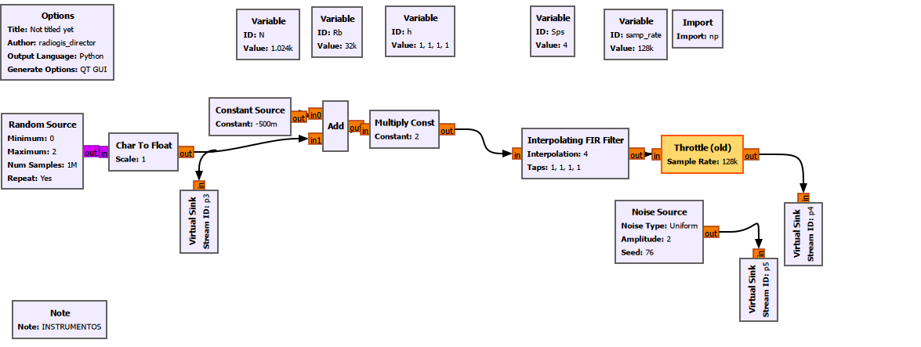
\includegraphics[width=1\linewidth]{DB1.png}
    \caption{Diagrama de bloques en GNURadio para las dos primeras etapas}
    \label{fig:DB1}
\end{figure}

\begin{figure}[H]
    \centering
    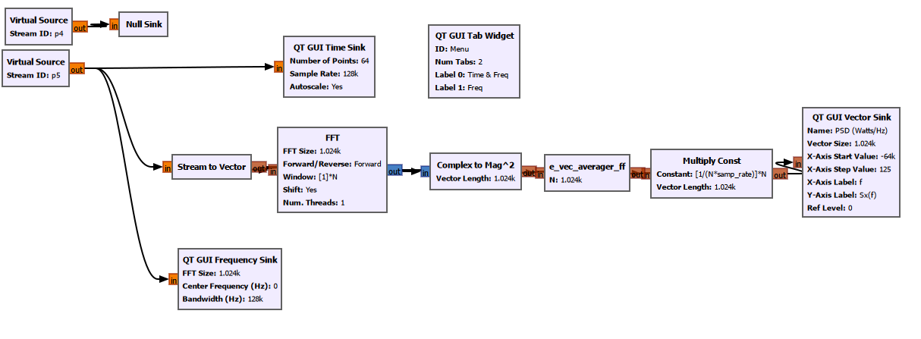
\includegraphics[width=1\linewidth]{DB2.png}
    \caption{Diagrama de bloques en GNURadio para estimar la PSD}
    \label{fig:DB2}
\end{figure}



\section{RESULTADOS Y ANÁLISIS DE DATOS}

\subsection{Análisis de la PSD variando el parámetro Sps}
Para el análisis de la señal binaria aleatoria bipolar de forma rectangular, se estableció una frecuencia de muestreo constante de $f_s = 128$ kHz. Se varió el número de muestras por símbolo ($Sps$) para observar su efecto sobre la tasa de bits ($R_b$) y el ancho de banda ($BW$). Teóricamente, la relación entre estos parámetros está dada por $R_b = \frac{f_s}{Sps}$ y el ancho de banda dado por $BW = 2R_b$.

\begin{table}[H]
\centering
\caption{Parámetros principales segun la variación de SPS}
\begin{tabular}{|c|c|c|c|}
\hline
\textbf{Sps} & \textbf{$f_s$ ($kHz$)} & \textbf{$R_b$ ($kbps$)} & \textbf{$BW$ ($kHz$)} \\
\hline
1 & 128 & 128 & 256 \\
\hline
4 & 128 & 32 & 64 \\
\hline
8 & 128& 16 & 32 \\
\hline
16 & 128 & 8 & 16 \\
\hline
\end{tabular}
\end{table}

\begin{figure}[H]
    \centering
    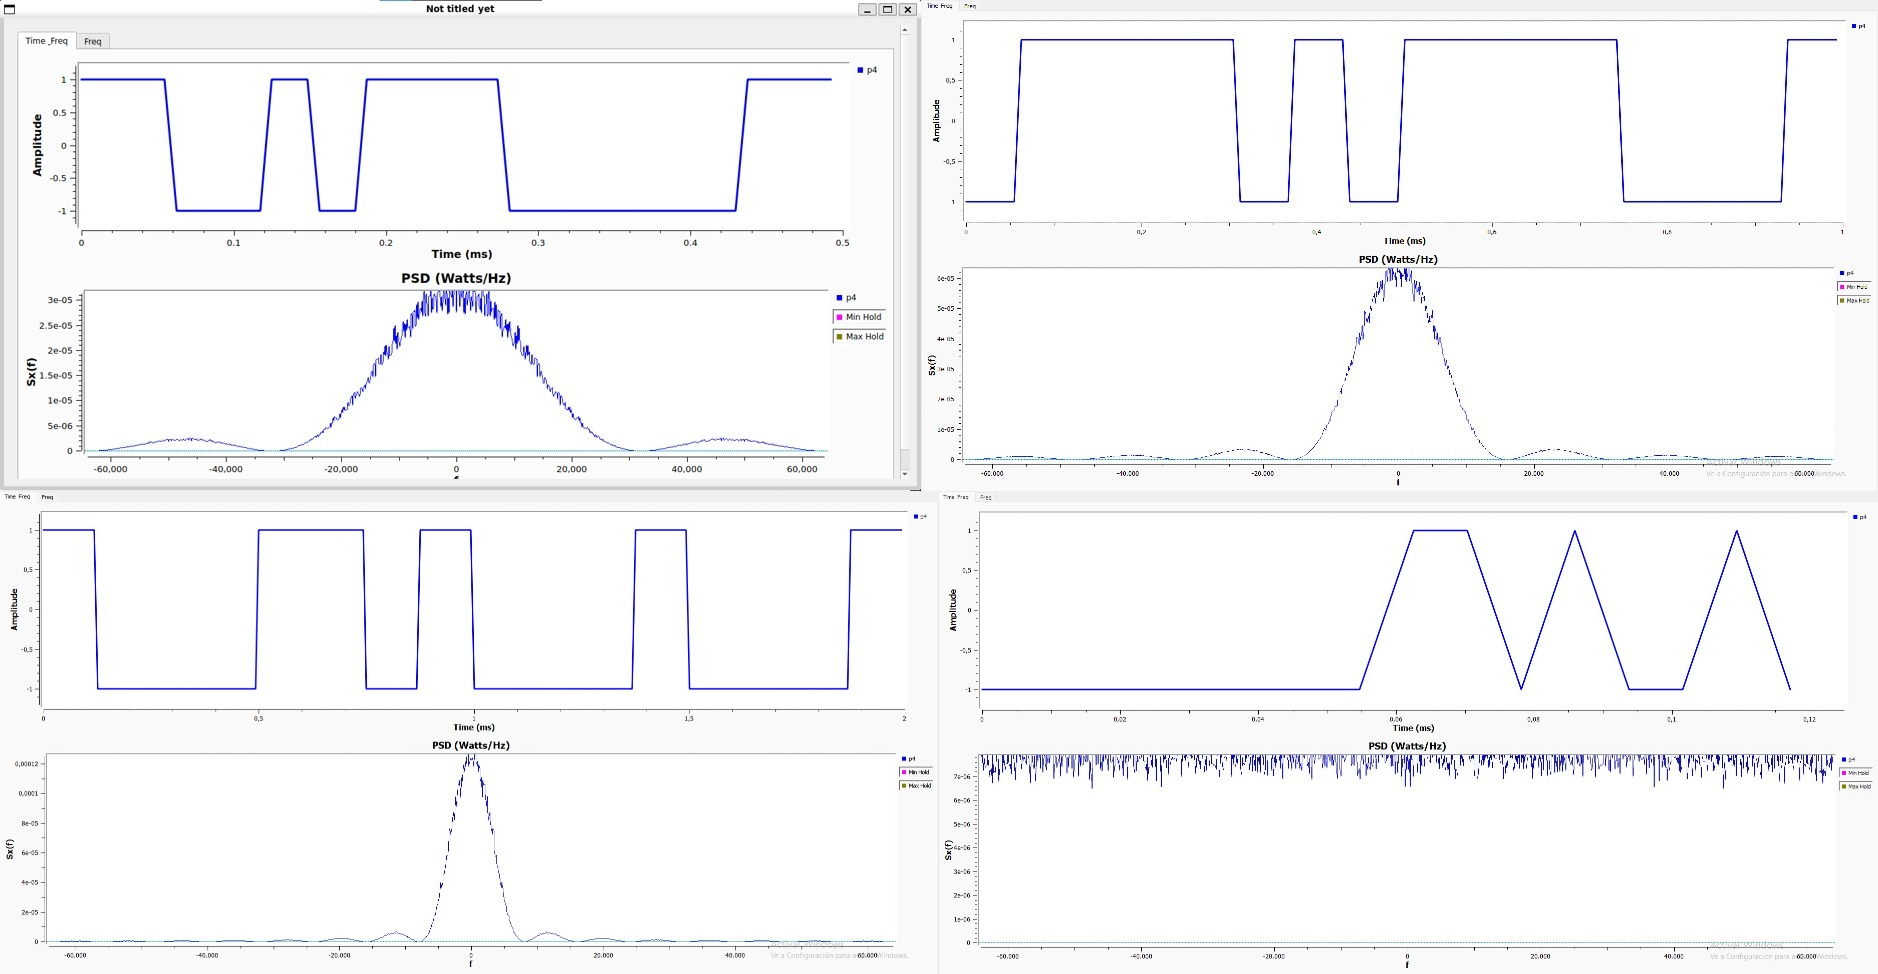
\includegraphics[width=1\linewidth]{image (2).jpg}
    \caption{Gráfica de la amplitud en el tiempo y de la PSD para distintos valores de Sps}
    \label{fig:SPS}
\end{figure}

Como se observa en la Figura \ref{fig:SPS}, existe una clara relación inversamente proporcional entre la duración del pulso ($T_b$) en el dominio del tiempo y el ancho de banda ($BW$) en el dominio de la frecuencia. A medida que el $Sps$ aumenta de $4$ a $16$, el pulso rectangular se ensancha (pasando de $0.03125$ ms a $0.125$ ms), lo que comprime el espectro y reduce progresivamente el ancho de banda del lóbulo principal de $64$ kHz a $16$ kHz, corroborando los cálculos teóricos. Por el contrario, el caso crítico se presenta con $Sps=1$, donde se tiene la duración más corta del pulso ($0.0078$ ms) y el ancho de banda se expande hasta $256$ kHz. En este último escenario, dado que la ventana de observación está limitada por el teorema de Nyquist, los cruces por cero no son visibles y la PSD adquiere un comportamiento lineal que se asemeja al del ruido blanco.

\subsection{Análisis de Ruido Blanco}

El ruido blanco se caracteriza por poseer una densidad espectral de potencia plana, indicando que su energía se distribuye de manera uniforme a través de todas las frecuencias del espectro. Para observar el comportamiento del ruido se dejo el $sps$ constante y solo se vario el ruido.


\begin{figure}[H]
    \centering
    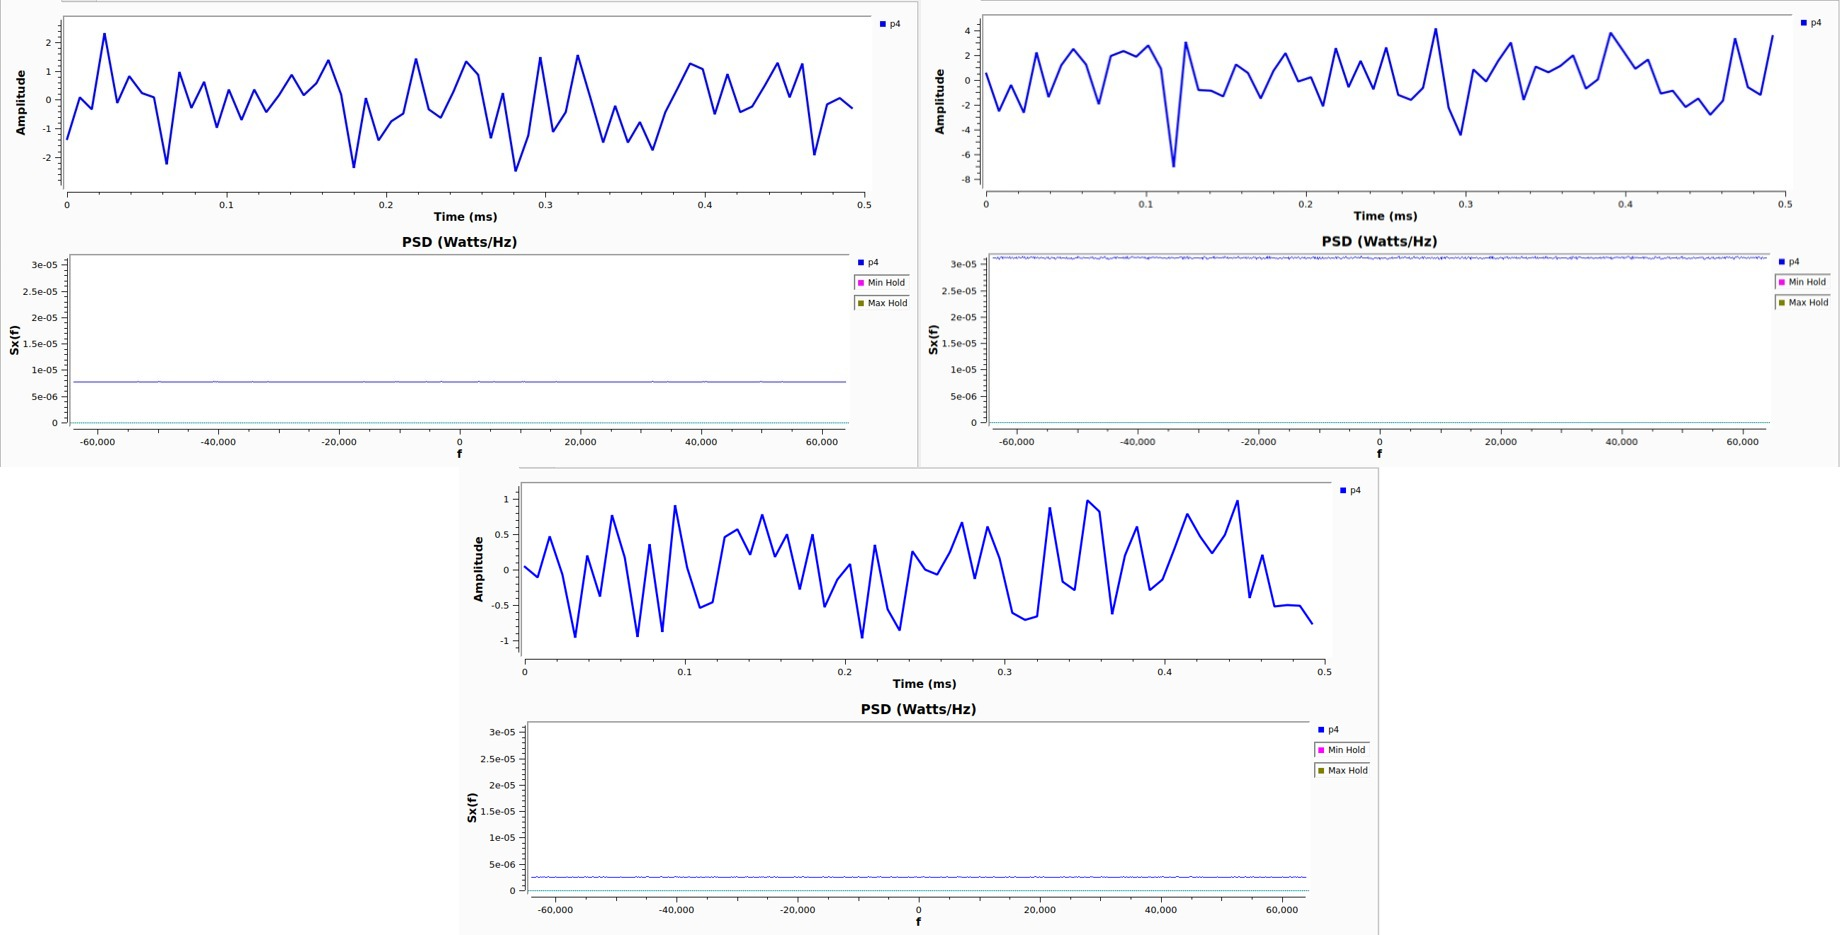
\includegraphics[width=1\linewidth]{image (4).jpg}
    \caption{Gráfica de la amplitud en el tiempo y de la PSD para distinto valores de ruido}
    \label{fig:RUIDO}
\end{figure}

Como se observa en la Figura \ref{fig:RUIDO}, al evaluar un ruido gaussiano con amplitud base de $1$, la señal temporal presenta variaciones con picos cercanos a $\pm 2.5$ y una PSD plana de aproximadamente $7.8 \times 10^{-6}$ W/Hz. Al incrementar la amplitud a $2$, la variación temporal se expande (con picos entre $4$ y $-8$) y, en consecuencia, el nivel espectral se eleva a $31 \times 10^{-6}$ W/Hz, conservando siempre su característica plana. Por otro lado, al cambiar la distribución de probabilidad a uniforme (con amplitud $1$), la señal temporal queda estrictamente en el intervalo $\pm 1$, perdiendo los picos aleatorios extremos propios de la campana de Gauss. A pesar de esta diferencia visual en el tiempo, la PSD continúa siendo una línea constante. Esto demuestra claramente que la naturaleza del ruido blanco depende de la uniformidad de su espectro y no de su distribución temporal. Observándose que en el último caso un nivel de PSD inferior, debido a que la varianza de la distribución uniforme es menor a la de la distribución normal.


\subsection{Entrada de imagen}

Al procesar la imagen \texttt{rana.jpg} mediante los bloques \textit{File Source} y \textit{Unpack K Bits}, la trama de bytes se convierte en un flujo binario no aleatorio transmitido en codificación polar NRZ ($\pm 1\text{ V}$). La Densidad Espectral de Potencia (PSD) resultante presenta la envolvente teórica tipo $\text{sinc}^2(f)$.

Para caracterizar exhaustivamente el sistema, se evaluaron tres variaciones fundamentales de parámetros:

\begin{itemize}
    \item \textbf{Efecto de repetición (\texttt{Repeat}):} Con \texttt{Repeat: Yes}, la lectura continua en bucle introduce una periodicidad $T_{\text{archivo}}$, generando líneas espectrales discretas (\textit{picket fence effect}) y fluctuaciones dinámicas en tiempo real. Por el contrario, con \texttt{Repeat: No}, la simulación procesa una ráfaga finita (\textit{burst}), estabilizando la PSD en una curva continua con rizado de ventaneo (\textit{ripples}) al finalizar el archivo.
    
    \item \textbf{Variación de la Tasa de Transmisión ($R_b$):} Al incrementar la tasa de bits $R_b$, el tiempo de bit $T_b = 1/R_b$ disminuye, provocando que la ráfaga de datos se procese en menor tiempo. En el dominio frecuencial, esto se traduce en una expansión proporcional del lóbulo principal de la PSD, desplazando los primeros nulos espectrales de $\pm 32\text{ kHz}$ a $\pm 64\text{ kHz}$ y confirmando la relación teórica $B_{\text{null}} = R_b$.
\end{itemize}

\begin{figure}[H]
    \centering
    \begin{subfigure}[b]{0.49\linewidth}
        \centering
        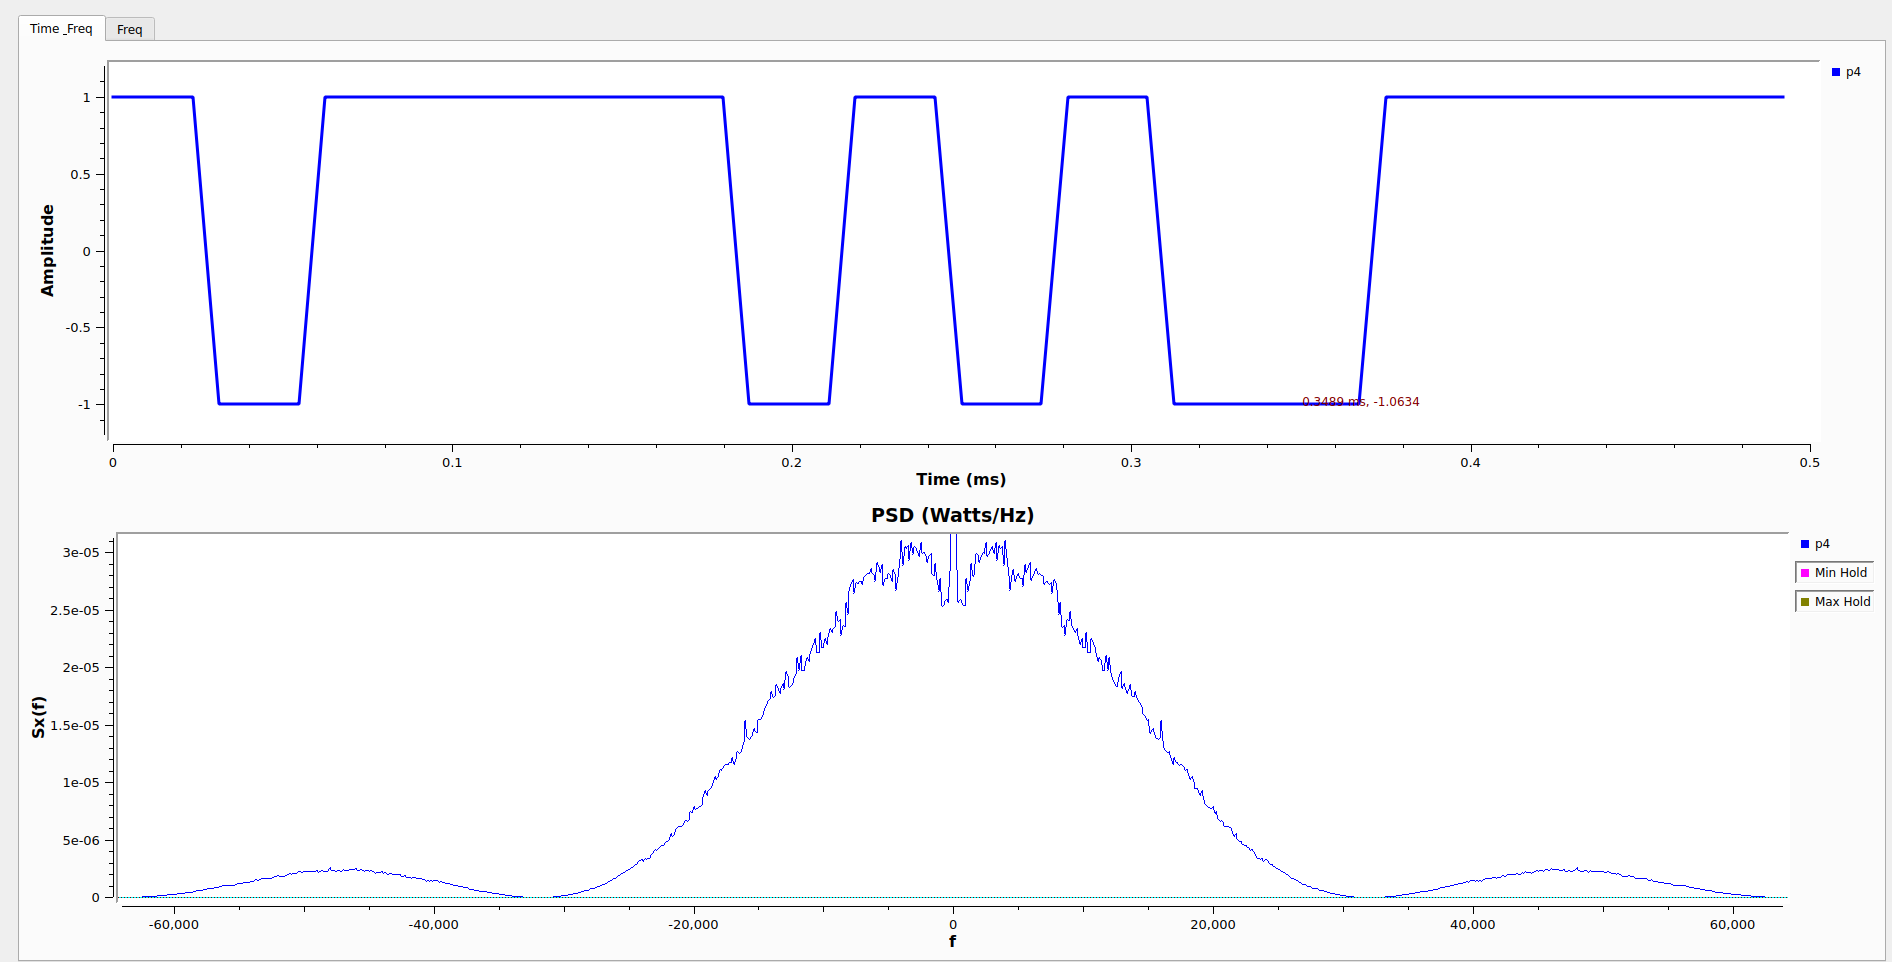
\includegraphics[width=\linewidth]{image_dec1d7.png}
        \caption{$R_b = 32\text{ kbps}$}
        \label{fig:rb_32}
    \end{subfigure}
    \hfill
    \begin{subfigure}[b]{0.49\linewidth}
        \centering
        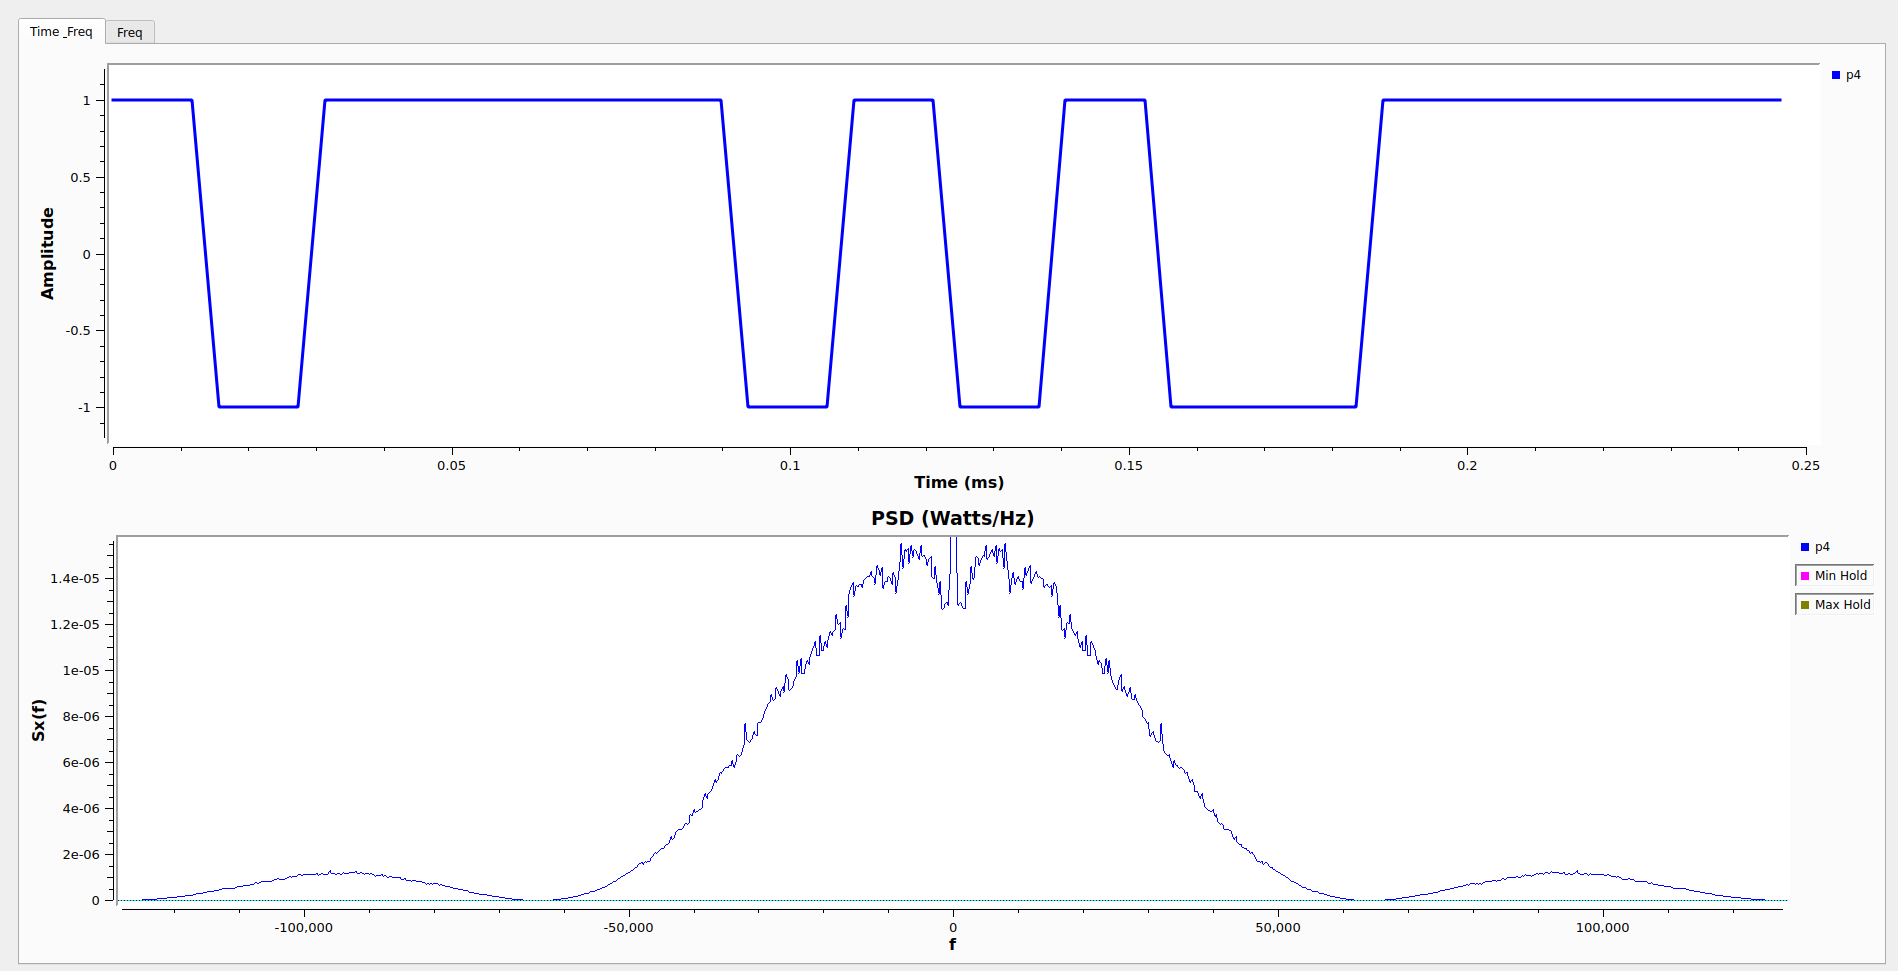
\includegraphics[width=\linewidth]{image_44642a.png}
        \caption{Incremento de $R_b$}
        \label{fig:rb_64}
    \end{subfigure}
    \caption{Respuesta temporal y espectral al variar la tasa de transmisión ($R_b$): (a) Configuración base con nulos en $\pm 32\text{ kHz}$. (b) Reducción de $T_b$ y expansión del lóbulo principal.}
    \label{fig:variacion_rb}
\end{figure}

\begin{itemize}
    \item \textbf{Variación de Muestras por Símbolo ($Sps = \text{len}(h)$):} Al modificar la longitud del vector $h$ para incrementar $Sps$ ($4 \to 8 \to 16$), la tasa de muestreo total $f_s = R_b \cdot Sps$ se eleva de $128\text{ kHz}$ a $512\text{ kHz}$. Esto expande la ventana del eje horizontal en el analizador de espectro ($\pm f_s/2$). Dado que el ancho de banda físico real de la señal depende únicamente de $R_b$, la PSD aparece visualmente más centrada y angosta, permitiendo observar más lóbulos secundarios de la función $\text{sinc}^2(f)$ sin atenuación ni distorsión por \textit{aliasing}.
\end{itemize}

\begin{figure}[H]
    \centering
    \begin{subfigure}[b]{0.49\linewidth}
        \centering
        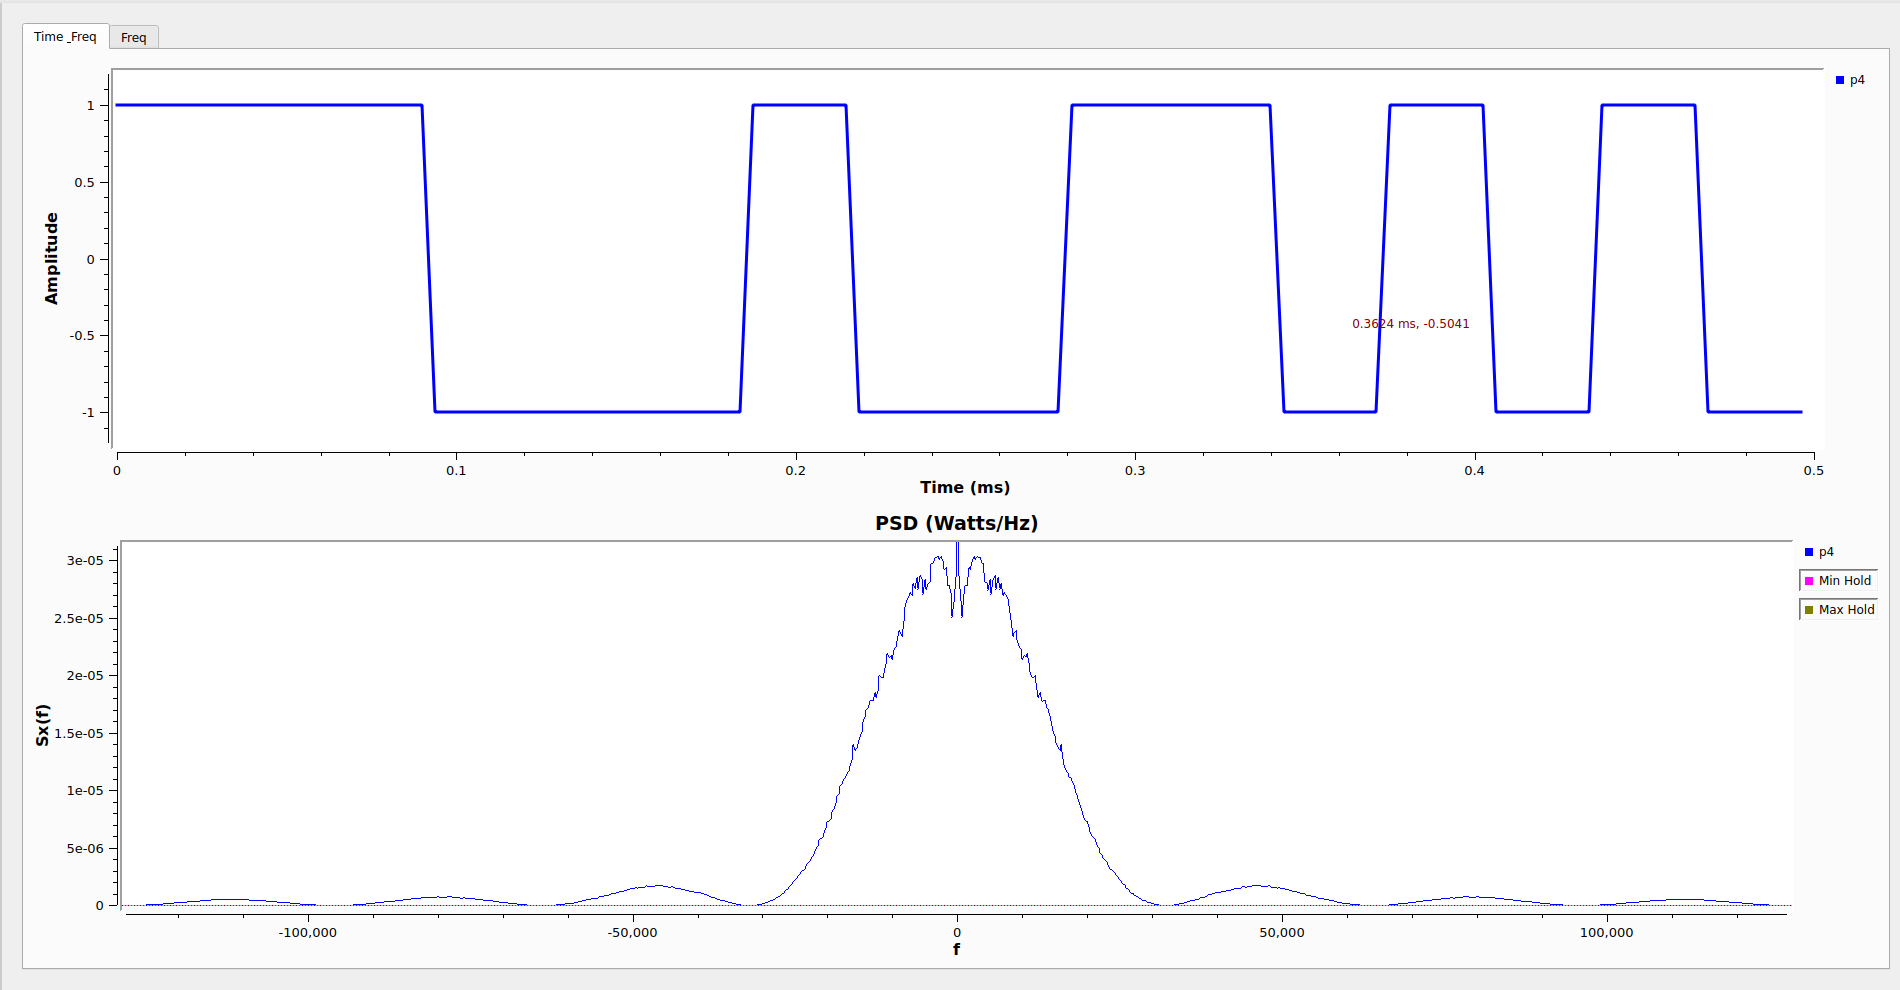
\includegraphics[width=\linewidth]{image_44d0ed.png}
        \caption{$Sps = 8$}
        \label{fig:sps_8}
    \end{subfigure}
    \hfill
    \begin{subfigure}[b]{0.49\linewidth}
        \centering
        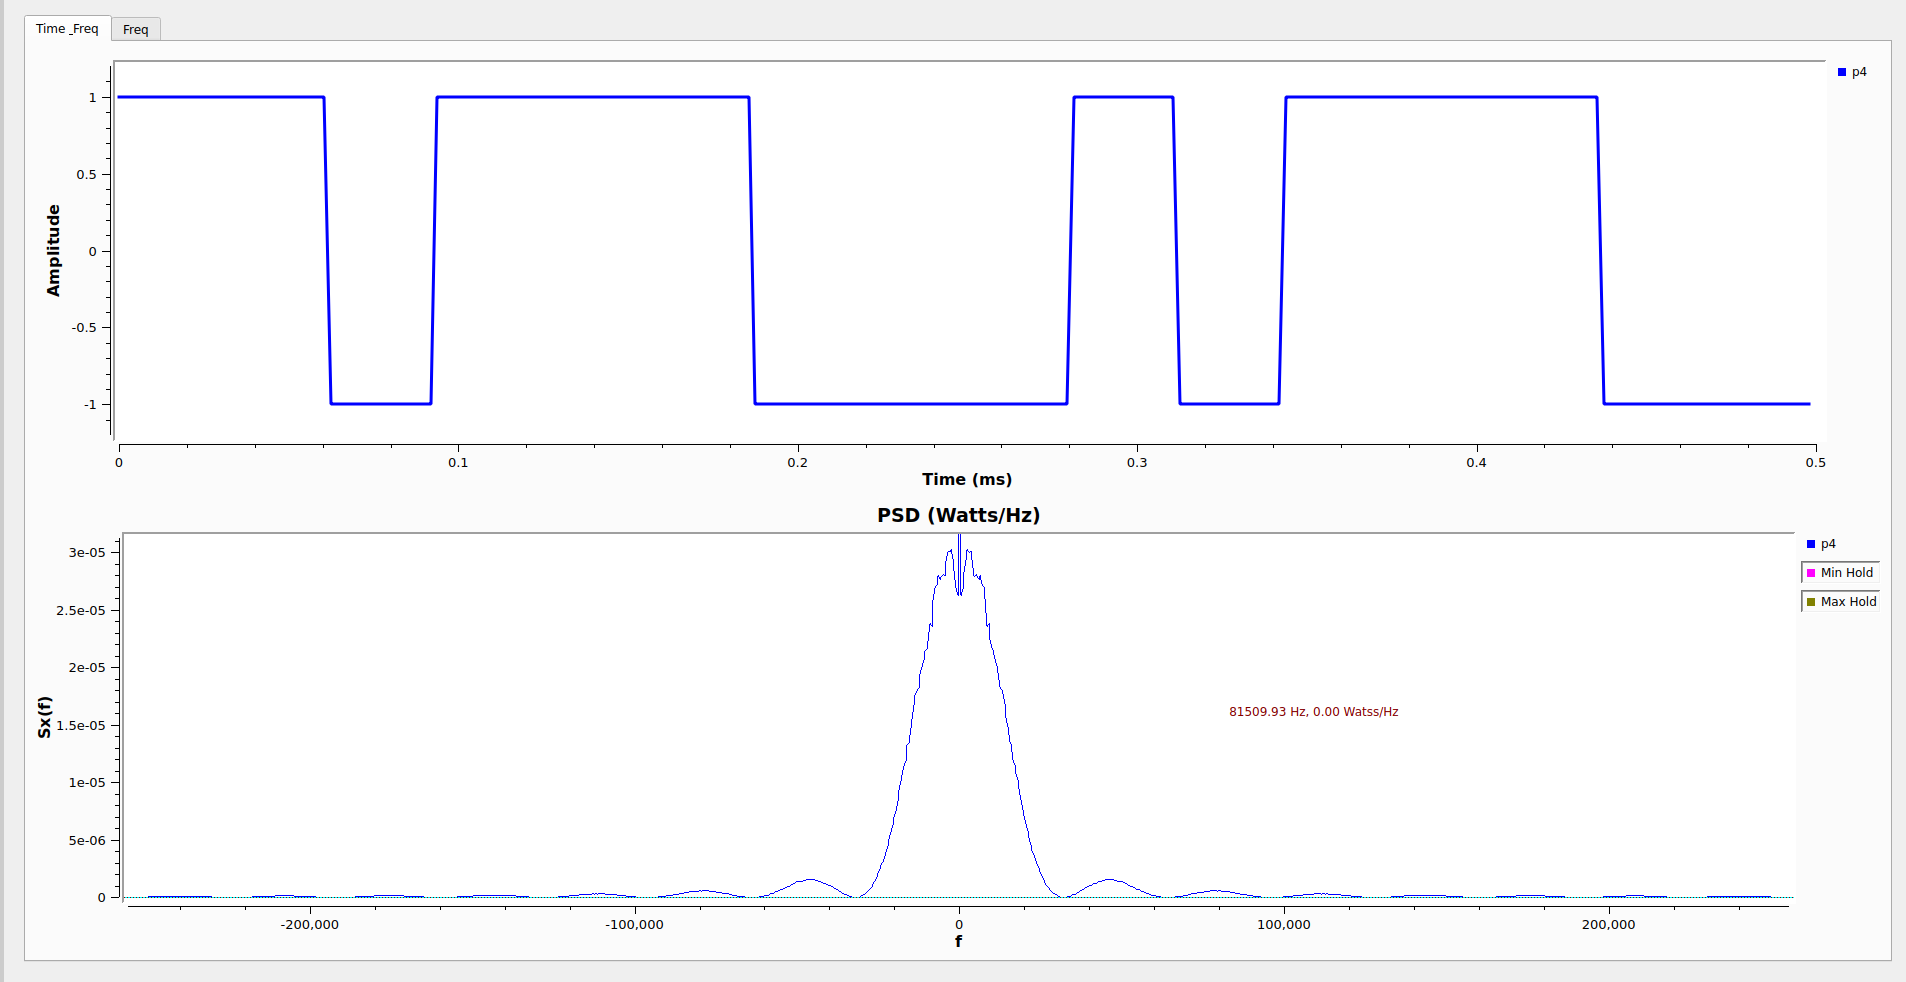
\includegraphics[width=\linewidth]{image_44d189.png}
        \caption{$Sps = 16$}
        \label{fig:sps_16}
    \end{subfigure}
    \caption{Efecto del sobremuestreo en la visualización espectral: (a) PSD con $f_s = 256\text{ kHz}$. (b) PSD con $f_s = 512\text{ kHz}$. Se evidencia la expansión del eje de frecuencias y visibilidad de lóbulos secundarios.}
    \label{fig:variacion_sps}
\end{figure}

% NO MODIFIQUE NI ELIMINE ESTA PARTE PARA QUE APAREZCAN LAS REFERENCIAS
\bibliographystyle{IEEEtran}

\begin{thebibliography}{00}

\bibitem{b1}
Escuela de Ingenierías Eléctrica, Electrónica y de Telecomunicaciones, 
\textit{Libro de Comunicaciones Plus Volumen I}. 
Bucaramanga, Colombia: Universidad Industrial de Santander, 2020, material de apoyo académico.


\end{thebibliography}

\end{document}